\documentclass[article]{IEEEtran}
\usepackage{cite}
\usepackage{color}
\usepackage{alltt}
\usepackage[utf8]{inputenc}
\usepackage{fancyvrb}
\usepackage{array} 
\usepackage{colortbl}
\usepackage{ctable}
\newcounter{tmpc}
\usepackage{mathtools}
\usepackage{widetext,amsmath}
\usepackage{subfigure}
\usepackage{caption}


\begin{document}
\title{Mapping Readers' Comments Back to Newspaper Articles}
\author{
        \IEEEauthorblockN{Asif Salekin, Md Anindya Prodhan, Muhammad Nur Yanhaona}
        \IEEEauthorblockA{	\\University of Virginia\\
                       		Email: \{as3df, mtp5cx, mny9md\}@virginia.edu}}
\maketitle


\maketitle
\begin{abstract}
Publishing readers' comments has long been an integral part of maintaining integrity in journalism. The evolution of electronic newspapers has greatly enhanced the scope and limit for these comments. So much so that now it is common to have hundreds of comments on popular issues in popular newspapers. The sheer volume of comments, however, introduces new challenges. For general readers it has become nearly impossible to go through all these comments. At the same time, for the newspaper editor it has become difficult highlighting comments most relevant to an article. 

In this project we worked on automatically filtering and mapping comments that are most relevant to a newspaper article or a portion of the article using information retrieval techniques. To be able to do that we analyse a newspaper article and construct query language models for terms that occurred in its passages. Then we generate queries from these passages and match them against readers' comments treating the latter as candidate relevant documents.

This report describes the logic and implementation of our solution, presents the first set of results we got from analysing some articles from two online newspapers, and discusses the problems we faced and possible future research directions.   
\end{abstract}


\section{Introduction}
Publishing readers' comments on newspaper articles has been a long-standing tradition in good journalism since the early days of newspaper. Sometimes such  comments convey readers' feelings about the original article; sometimes they provide complementary information that help other readers to get a holistic understanding of the discussed topics; sometimes they expose errors, omissions, or subtle bias on the part of the reporter; and so on. Publication of readers' comments has, therefore, become an integral part of transparency in journalism.

During the era of printed newspapers, these comments used to appear as follow-up  discussions in days following the date of original article publishing. Because of space constraints, follow-up comments tend to be limited to only a few interesting news and furthermore limited in their numbers. The advent of electronic newspapers, however, has fundamentally altered that pre-existing culture. Currently, comments can be written on every published articles, by anyone interested,  and there is no limit in the number of comments either. Now it is quite common to see several hundreds of comments on popular news articles in papers, like, New York Times and BBC News.

In regards to fact finding and ensuring transparency this is an encouraging trend. The sheer volume of such comments, however, introduces several important  challenges. On one hand, it can be overwhelming or completely unreasonable for a common reader to go through all the comments. On the other hand, for the editor it is difficult to highlight comments that may be most relevant to the  original article or purge comments that are simply vile. To the best of our  knowledge, so far little has been tried to aid both parties in this regard by automatic highlighting, filtering, and classification of readers' comments.

Although our broad objective for this research was to address all of the above, as part of the class project we focus on filtering relevant comments only. The central idea behind our solution is to view an article title as a query and the article itself as a feedback document for constructing the language model for the query intended by the title. Then to judge relevance of comments to the article or passages in the article, we automatically generate queries from the constructed model and rank comments against them.       

For our experiment we crawled about 1000 articles each having at least 20 comments from Alzajeera News and collected 780 more similarly comment-rich articles from Yahoo-News gathered by authors of \cite{Das:2014:GBC:2556195.2556231}. Language models for articles are uni-gram models that we generated using our own algorithm that relies on a notion of term significance which depends on both frequency and proximity of terms related to terms in the article title. Then a corpus based smoothing is applied to determine final term significance rankings. In short, a model in our case is not just a collection of terms; rather a probability estimate is associated with each term regarding its chance to be included in a query representing the information need served by the article or a part of that article. 

Ranking of comments against generated queries is done using Okapi BM25 \cite{Robertson96okapiat}. We varied different parameters of the ranking function as well as of our term significance calculation algorithm to identify the best configuration. The ground truth for comments' relevance is gathered through human evaluation of a small random sample of news from our crawled database.

The results are encouraging. Nevertheless, we identified several challenges regarding improving our solution further. Some problems were implementation specific issues that arose from simplifications we had to make to save time. There are good reasons to be optimistic and we hope to enhance our solution in the future.  

\subsection*{Report Organization}
The rest of the report is organized as follows. Section \ref{rw} discusses some related work; Section \ref{pf} describes how we model our domain as an information retrieval problem; Section \ref{des} elaborates on fundamental design aspects of our solution; Section \ref{si} briefs on the actual implementation; Section \ref{ev} presents the results of the experiment done on a small sample of articles; Section \ref{fw} ponders over possible routes for future work; finally, Section \ref{con} concludes the report.                

\section{Related Work}
\label{rw}
There have been a few works done on matching comments with news article segments. Sil et. al. \cite{Sil:2011:SMC:2063576.2063906} used supervised and unsupervised techniques to create structural classifiers to match comments with news article segments. Their paper used explicit semantic analysis and co-reference features to represent the text in article and showed that the accuracy of discriminative approaches depends largely on effective feature selection. They used prior data to detect article segments and matched comments in articles based on related topics.

Our algorithm for generating language models from an article has some parallel to topic modelling of documents. Several works have been done regarding topic modelling. MG-LDA \cite{Blei:2003:MAD:860435.860460, Titov:2008:MOR:1367497.1367513} is used to model local topics in a text. In a news article every segment may not be related to a comment. Also in this model, local topics scatter across the corpus which is not often the case in news articles. Hence, MG-LDA is not appropriate for our system. 

Corr-LDA \cite{Titov:2008:MOR:1367497.1367513} is another topic model to understand correspondence. Since, Corr-LDA work with single vector model, a specific comment on a small segment of an article can show small correlation with the article using this model. To overcome this limitation Das et. al. \cite{Das:2014:GBC:2556195.2556231} developed a correspondence topic model (SCTM) that uses multiple topic vectors. Hence, for each comment-article segment pair there would be a number of topic vectors, which would enable comments to match with more correspondence segments of article. 

In \cite{Ma:2012:TRC:2396761.2396798} the authors focused on summarizing comments. This paper selects few most representative comments from comment cluster for an article. They used Master-Slave Topic model (MSTM) and Extended Master-Slave Topic model (EXTM) where News articles is treated as master and comment text as slave. Using this topic models they cluster the comments based on their topics and rank the most representative comments from each comment clusters. One significant limitation of their work is that they assumed that a comment is related to a single topic exclusively. 

Since our criteria for filtering and categorizing comments under article segments significantly differ from the objectives of aforementioned works, there is considerable novelty in our solution. For example, none of the works we came upon use the structure of a news article into consideration to construct its models. We are unaware of any previous work that uses query generation techniques to match comments against their underlying newspaper articles.       

\section{Problem Formulation}
\label{pf}
This section describes how we model the problem of finding relevant readers' comments as an information retrieval problem.

We view components of a news -- consisting the article and associated comments --  to serve a single information need. This information need can be thought of as represented by a query that is similar to the title of the article. In our formulation, comments are of interest only because the original article is insufficient in conveying all information necessary to fully satisfy a reader's information need all by itself. 

Given this formation, comments of interest are those comments that address topics covered in the article but augment article's author arguments in some way. These comments broadly fall into two categories.  

\begin{enumerate}
\item Comments that support article author's arguments with additional information and insights, and
\item Comments that contradict the article with contradictory evidences and insights
\setcounter{tmpc}{\theenumi}
\end{enumerate}

Given the unregulated nature of comments publishing, the Comments Section of the news is often cluttered with several other kinds of comments such as (as we observed)

\begin{enumerate}
\setcounter{enumi}{\thetmpc}
\item Comments that express nothing but readers' sentiments about discussed topics
\item Exchange of arguments among readers about each other's comments
\item Elaborate discussion on some offshoot topic that has minute relevance to the article itself
\end{enumerate} 

An abundance of comments of latter categories makes it difficult for an unbiased reader to identify and consequently satisfy his partially fulfilled information need. Although distinguishing between the former and latter kinds of comments is often a subjective decision, henceforth difficult, we hold that comments of former categories are more likely to have the following characteristic that will separate them out from the latter.
\bigskip

\textit{There is significantly larger overlapping between principal issues discussed in an article and in a relevant comment than between the article and a non-relevant comment.}    
\bigskip

Given this assumption, the problem of filtering relevant comments can be designed as a standard information retrieval problem that has two parts.

\begin{enumerate}
\item Construct query language models from passages of an article 
\item Generate queries from these models and rank comments against individual queries
\end{enumerate}

Here we consider passage specific models as for articles having many passages, there may be jump in the topics been discussed. Consequently, a comment may also have passage specific complementary discussions. In the general case, the article represents a composite language model that is a mixture of the models of individual passages; and in the degenerative base case, it represents a single passage itself.  

Before we dive into a discussion about our implementation, we should emphasize that our language model should not be equated to a topic model present in some related work discussed previously. Rather, it is intended to generate queries. To clarify the difference with an example, if ``Obama decided to go alone in the Immigration reform issue" is a title of a news article then from the topic modeling perspective ``Immigration Reform'' is the primary -- and arguably the sole -- topic but from the query generation perspective ``Obama's Decision'' alongside ``Immigration Reform'' should construe the crux of the discussion.    

\section{The Design}
\label{des}
The center piece of our solution is the algorithm for developing query language models for individual passages of a newspaper article. Next we discuss the algorithm. Afterwords we discuss how these models can be used to generate queries that would be used for ranking evaluation.   

\subsection{Query Model Generation}
Given that we treat an article title to be equivalent to a query representing readers' information need, we have a mechanism to interpret the significance of the content of the article. We believe a reasonable interpretation for any article is that each passage provides a partial information about the issue underlying the title and each sentence within a passage works on building up the argument of its passage. To summarize, their is no term in the article that is not relevant to readers' information need.     

The relevance of these terms are, however, different and based on several parameters given below. 

\begin{enumerate}
\item Term Frequency
\item Significance Level: the minimum distance of a term from terms occurring in the title
\item Relevance Weight: the number of co-occurrences of a term with other significant terms in the article 
\item Smoothing Factor: general likelihood of appearance of the term within the corpus      
\end{enumerate}

Among these the first and the last are self explanatory. So we focus on explaining the remaining two.

To calculate both significance level and relevance weight of terms we construct a graph ${G = (V, E)}$ for each passage $P$ where the vertex set is defined as, $V = \{w_i | w_i \in P\}$; and the edge set as, $E = \{(w_i, w_j) | w_i, w_j \in s_k, s_k \in P\}$. That is there is an edge between two words if they occur in the same sentence anywhere in the passage. Here co-occurrences in multiple sentences results in multiple edges. 

Then the formula for the significance level of a word $w_i$ is as follows, 
\begin{equation}
\begin{array}{lr}
s_i = 1 : w_i \in title \\
s_i = 1 + distance_{min}(w_i, w_j) | w_j \in title) : w_i \notin title
\end{array}
\end{equation}
Here distance is measured as the number of edges between the concerned words pair.  

The formula for the relevance weight of a word $w_i$ is as follows, 
\begin{equation}
\label{rwEq}
rWeight_i = \sum_{\substack{(w_i, w_j) \in E\\s_j < s_i}} max\big(0, 1 - \log(s_j)\big)
\end{equation}
 

If we reason about aforementioned formulas, we see that terms that occurred at close proximity of terms in the title have more significance than terms that appeared further. Then terms that occurred more often and with more significant terms have more relevance weight than terms that occurred less often.  

The rationale for this treatment lies in the assumption about the logical flow of arguments that we expect to present in a newspaper article. Sentences making statements about elements of the title should compose the main agenda. Then there will be sentences providing supporting evidences and so on. Consequently, terms occurring in different kind of sentences should have varying degrees of importance in the constructed model.   

Note that in Equation \ref{rwEq} only the term with lesser significance, $w_i$, gets the benefit of co-occurrence -- not the term with greater significance, $w_j$. This apparent lacking is balanced by the frequency weight of individual terms which has the following formula.

\begin{equation}
\label{fweight}
fWeight_i = tf \times {\frac{s_i + k}{s_i (k + 1)}}
\end{equation}   
Here $k$ is a scaling parameter used to exponentially decrease the importance of a term's occurrences with increase of its significance level.
The likelihood of a term to contribute to a query representing the information need satisfied by the concerned passage of the article is calculated as a mixture of normalized relevance and frequency weights as captured by the following equation.

\begin{equation}
\label{docW}
weight_i = \alpha \times rWeight_i^{norm} + (1 - \alpha) \times fWeight_i^{norm}
\end{equation}

Equation \ref{docW} is combined with the collection probability of a terms $p(w_i, C)$ using the Jelinek-Mercer interpolated smoothing method \cite{1371580} to give the final smoothed probability as follows.   

\begin{equation}
\label{wProb}
p_q(w_i) = (1 - \lambda) \times weight_i + \lambda \times p(w_i, C) 
\end{equation}



\subsection{Ranking Evaluation}
If we remember the discussion of Section \ref{pf}, we see that the criteria for judging relevance of a comment to the discussion presented in the article or a passage of the article is the degree of overlapping of comment's language model with that of the latter. Here \textit{overlapping} deserves careful attention.

Note that we expect from a relevant comment to complement the discussion of the article with supporting or contradictory arguments. We do not expect the comment to say the same thing the article does. So there should be significant overlapping in principal terms of the comment and the article, but there should also be considerable distinction in their auxiliary terms. Therefore, ideally the goal of comments ranking should not be to maximize overlapping. Rather it should be to balance similarity in principal terms with dissimilarity in auxiliary terms.

\begin{figure*}[!ht]
\centering
\captionsetup{justification=centering}
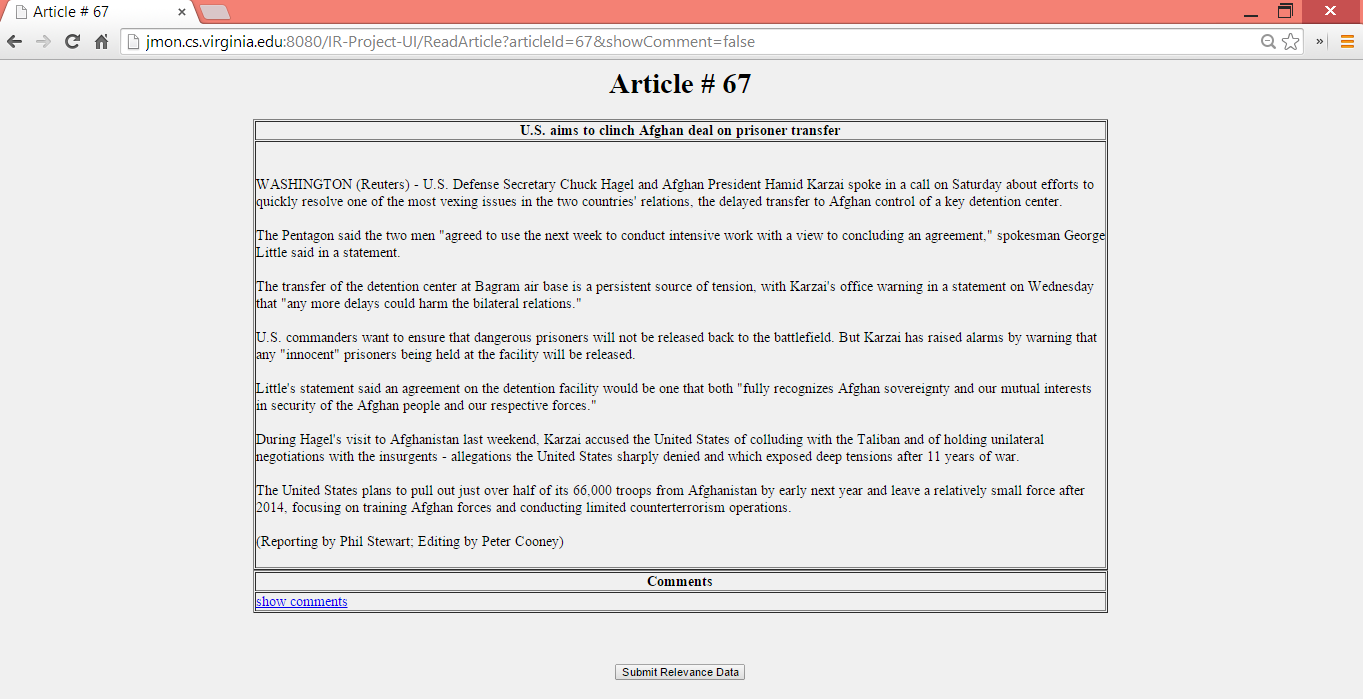
\includegraphics[trim=0cm 0cm 0cm 0cm, clip=true, totalheight=0.5\textheight, angle=0]{feedback-1.png}
\caption{\textbf{User interface to provide feedback}} \label{feedback}
\end{figure*}


If we define a cut-off threshold for partitioning the query language model of a passage $P$ into a principal $\theta_{pri}$ and an auxiliary part $\theta_{aux}$ then the relevance judgement for a comment $D$ with respect to the passage can be expressed as a harmonic mean as follows.

\begin{equation}
\label{relMes}
relevance(P,D) = \frac{1}{\frac{\beta}{sim(\theta_{pri}, \theta_d)} - \frac{1 - \beta}{sim(\theta_{aux}, \theta_d)}}
\end{equation}           



This is a generic equation and any standard metric -- for example KL-divergence -- can be substituted as the similarity measure to calculate the relevance in the above.

A reasonable simplification to Equation \ref{relMes} is to consider only the similarity between the comment model and passage model in the principal terms. This is practical as it is highly unlikely that a comment will only reiterate the argument presented in an article. Hence we can ignore the dissimilarity term and rank comments based on the following formula.

\begin{equation}
\label{rank}
rank(P,D) \sim sim(\theta_{pri}, \theta_d)
\end{equation} 



\section{Implementation}
\label{si}
We made a few modifications to the solution described in the previous section for practical considerations and -- particularly -- to save time. As we will discuss actual implementation in this section, these deviations will become apparent.   

We use Apache OpenNLP parser \cite{openNLP} to extract sentences from the article then to determine parts of speech of all words in the article. Then we keep only the nouns and verbs for later analysis. We make this decision as our observation indicates that conjunctions, prepositions, and adverbs usually have little to contribute to the central arguments of an article; and our collection of articles is not large enough to nullify their influence by applying smoothing alone. We are uncertain about the import of adjectives and currently leave them out. Our system is configurable though and different parts of speech can be enabled and disabled in it if deemed useful.

For passage identification, we adopt the simple strategy that a paragraph with a minimum $n$ sentences portrays a holistic argument/evidence and a sequence of $m$ such paragraphs form a passage. If a paragraph is less than $n$ sentences than we consider it to be automatically included in the current passage without increasing passage's paragraphs count. Our original plan was to try different combinations of $n$ and $m$ and determine what performs best. To our surprise, the vast majority of news articles seem to have paragraphs that are mostly one or two sentences long. Hence in most cases, we get only one passage, consequently one query model, per article. There are exceptions though.                     

The query language model is implemented exactly according to the formulas given in the previous section using our own data structures and algorithms. The pairwise term association graph is implemented combining two map data structures that are generated using words tagged and filtered during parsing phase. Then frequency and relevance weights are measured concurrently by traversing the graph starting from the title words. Finally they are normalized. The time and space complexities for the algorithm are $\mathcal{O}(|E|)$ and $\mathcal{O}(|V| + |E|)$ respectively.

Computing the collection (or corpus) model is the costliest part because we have to analyse all articles. That is however computed only once and the model is been stored in a file. Before ranking, the model is been loaded in memory and used as many times as required. Note that we keep separate collection models for articles coming from different news websites. This is to capture the writing style and vocabulary differences that we observe when reading articles from different news sources. Our original plan was to further partition the collections based on news categories as it is reasonable to expect to see differences in frequent terms as we shift reading articles from, say, sports to politics. We did not do that at the end as our collections of news per category were not large enough.     

The biggest sacrifice that we have to make concerns about ranking evaluation. This happened regrettably because of time constraint due to our engagement in other research. We used Apache Lucene \cite{McCandless:2010:LAS:1893016} for indexing comments of an article and ranking them against our generated query model. Since we could not manage time to study and implement a language model based ranking process over Lucene as that would be required by Equation \ref{rank}, we directly generate a query from the model selecting terms with high weights and 
rank comments against this query using Okapi BM25 \cite{Robertson96okapiat}.

\begin{figure*}[!ht]
\centering
\captionsetup{justification=centering}
{\subfigure[ MAP Varying $\alpha$ ]{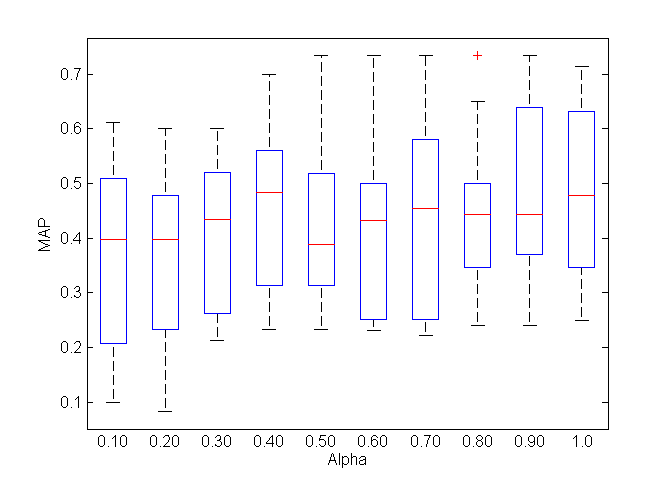
\includegraphics[trim=0cm 0cm 0cm 0cm, clip=false, totalheight=0.3\textheight, angle=0]{alpha-map.png}%
\label{alpha-map}} \hfil 
\subfigure[ P@5 Varying $\alpha$ ]{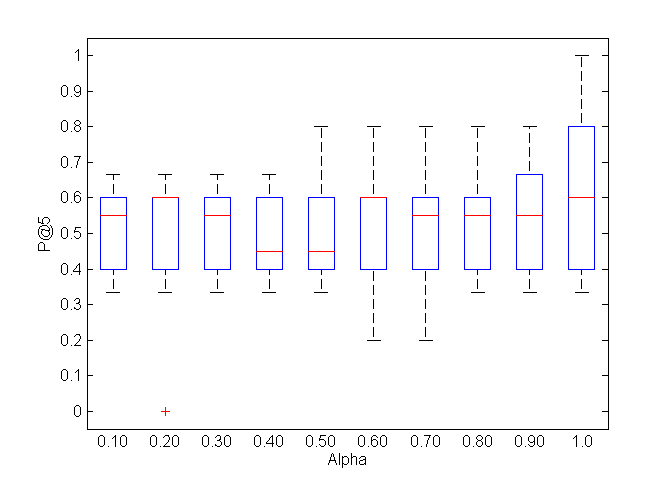
\includegraphics[trim=0cm 0cm 0cm 0cm, clip=false, totalheight=0.3\textheight, angle=0]{alpha.png}%
\label{alpha-p5}}} \caption{\textbf{Two different performance measure(MAP and P@5) were computed for different values of $\alpha$. For these experiments the others parameters were as follows: $\lambda$ = 0.9, terms = 70, $b$ = 0.1}} \label{alpha}
\end{figure*}


This adjustment has the shortcoming that the probabilities for principal terms available in the query model have been used during query generation, but the advantage of their presence has not been taken during ranking comments as the ranking function treats all query terms to be equal. We suspect this has a significant adverse effect in our solution's performance. We hope to correct this problem in the future -- depending on the feedback we may get regarding the future prospect of this work.       
     

%\begin{figure*}[!ht]
%\center{\subfigure[ An Article ]{\includegraphics[trim=0cm 0cm 0cm 0cm, clip=false, totalheight=0.25\textheight, angle=0]{snapshot1.png}%
%\label{res1}} \hfil 
%\subfigure[ The comments to provide feedback ]{\includegraphics[trim=0cm 0cm 0cm 0cm, clip=false, totalheight=0.25\textheight, angle=0]{snapshot2.png}%
%\label{res2}}} \caption{User interface to provide feedback} \label{results}
%\end{figure*}

\section{Evaluation}
\label{ev}
In order to evaluate our system, we asked some of our peers to read a few articles from our crawled Alzajeera and Yahoo-news archive and requested them to provide feedback specifying which of the comments associated with the article are relevant. We implemented a web interface  to acquire user feedback. Figure \ref{feedback} presents a snap-shot of our user interface. We gathered 10 feedback for Alzajeera news articles and 10 feedback for Yahoo-news articles. These feedback were used as our ground truth for our evaluation.  

We conducted our evaluation in two-phases. At the first phase, we used the feedback  for Alzajeera news articles as our training set to determine the optimal value for all the parameters discussed in the previous section. At the second phase, we used these parameters to evaluate the performance of our system with Yahoo-news articles.

We used two very well known performance measures for information retrieval: MAP (Mean Average Precision) and P@5 (Precision at position 5). As one of the motivation of the project was to present an editors' pick of comments (typically 5 of the best comments are selected as editors' pick), we choose to use P@5 to evaluate our system. MAP would present an overall performance of our system in terms of precision and recall.

\subsection{Identifying the best Parameters}
\label{best-param}
In our proposed approach, we have used several different parameters, such as the parameter $k$ in Equation \ref{fweight}, parameter $\alpha$ in Equation \ref{docW} and parameter $\lambda$ in Equation \ref{wProb}. Also, BM25 have length normalization parameter ($b$), and other parameters like $k_1$, $k_2$. Also, we can vary the number of terms generated in our query generation process. In order to identify the best parameters, we tried to vary each of these parameters individually while keeping all other parameters constant. Our results show that the parameters $k$, $k_1$ and $k_2$ don't have much of an impact on the MAP and P@5 value. So, in this section, we present the results of varying other four parameters to get their best possible value.

\subsubsection{$\alpha$}
Equation \ref{docW} is a mixture of normalized relevance and frequency weights. It gives the likelihood of a term to appear in the query for the concerned passage of the article. Figure \ref{alpha-map} and Figure \ref{alpha-p5} shows impact of change in $\alpha$ on MAP and P@5 respectively. For the experiment the value of the other parameters were fixed as $\lambda$ = 0.9, terms = 70, $b$ = 0.1.

From Equation \ref{docW}, we see that, if the value of $\alpha$ is close to 0, relevance weight will have very low impact on term likelihood to appear in query. If value of $\alpha$ is close to 1, frequency weight of individual terms will have very low impact on likelihood to appear in query.  Figure \ref{alpha} shows that, both P@5 and MAP increase with increase of $\alpha$ which indicates that, relevance weight should have more significant impact on term likelihood to appear in query for the concerned passage of the article. So for the rest of the experiments we set the value of $\alpha$ as 1.0.


\subsubsection{$\lambda$}
\begin{figure*}[!ht]
\centering
\captionsetup{justification=centering}
{\subfigure[ MAP Varying $\lambda$ ]{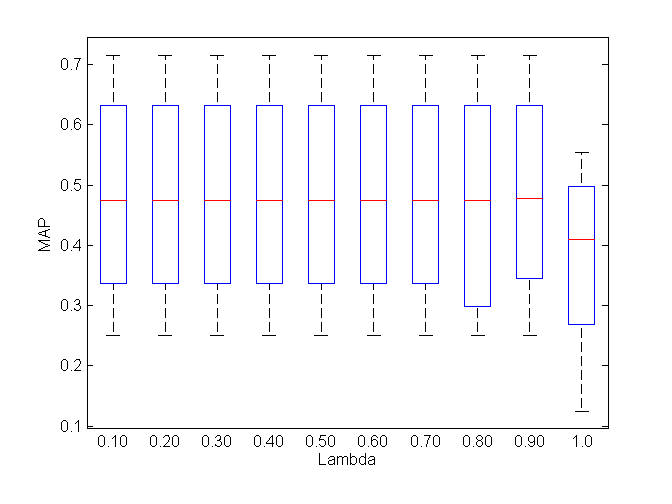
\includegraphics[trim=0cm 0cm 0cm 0cm, clip=false, totalheight=0.3\textheight, angle=0]{beta-map.png}%
\label{lambda-map}} \hfil 
\subfigure[ P@5 Varying $\lambda$ ]{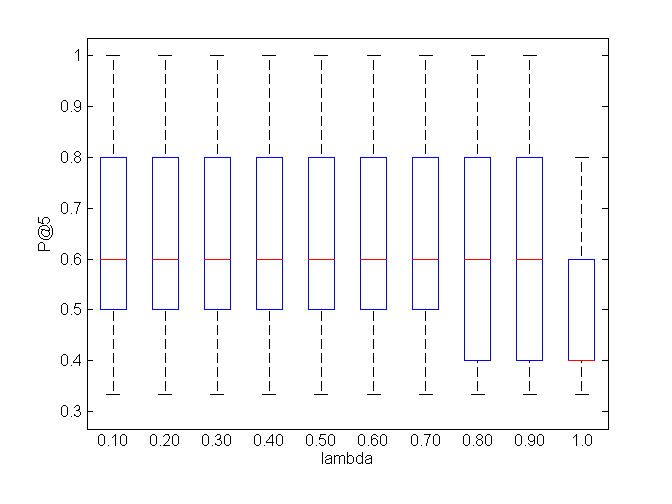
\includegraphics[trim=0cm 0cm 0cm 0cm, clip=false, totalheight=0.3\textheight, angle=0]{beta.png}%
\label{lambda-p5}}} \caption{\textbf{Two different performance measure(MAP and P@5) were computed for different values of $\lambda$. For these experiments the others parameters were as follows: $\alpha$ = 1.0, terms = 70, $b$ = 0.1}} \label{lambda}
\end{figure*}
Equation \ref{wProb} combines the term likelihood to appear in query for the concerned passage of the article with the collection probability of a term $p(w_i,C)$ using the Jelinek-Mercer interpolated smoothing method. In this equation the smoothing parameter is $\lambda$. Figure \ref{lambda-map} and Figure \ref{lambda-p5} shows the change of MAP and P@5 with the change of the smoothing parameter $\lambda$. For these experiments, the values of terms and $b$ were set to 70 and 0.1 respectively.

Figure \ref{lambda} shows that MAP and P@5 both remains almost similar for values of 0 to .9 for $\lambda$. We get highest MAP of .4804 for $\lambda$ value of 0.9. MAP decrease significantly if $\lambda$ is 1. However, as the smoothing probabilities ($p(w_i,c)$) are so small that we typically can't get any effect of smoothing unless we set a higher value for $\lambda$. For this reason, for the rest of the evaluation we selected the $lambda$ as 0.9.

\subsubsection{Doc Length Normalization for BM25}
\begin{figure*}[!ht]
\centering
\captionsetup{justification=centering}
{\subfigure[ MAP Varying the parameter $b$ ]{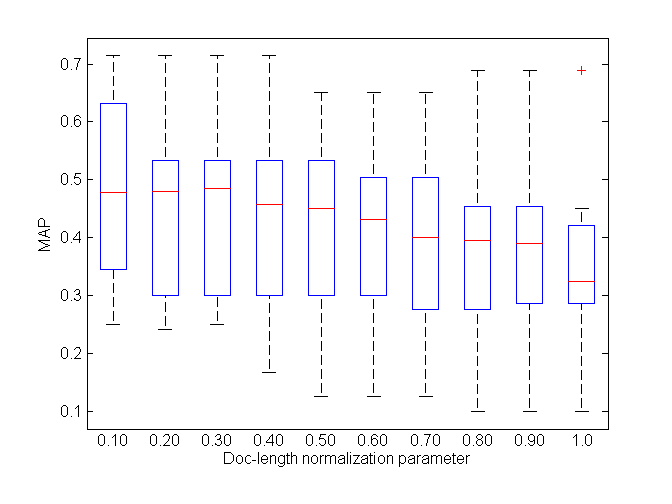
\includegraphics[trim=0cm 0cm 0cm 0cm, clip=false, totalheight=0.3\textheight, angle=0]{b-map.png}%
\label{b-map}} \hfil 
\subfigure[ P@5 Varying the parameter $b$ ]{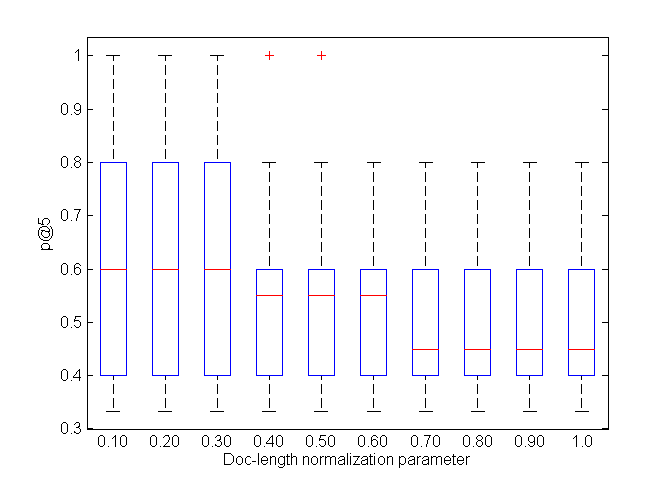
\includegraphics[trim=0cm 0cm 0cm 0cm, clip=false, totalheight=0.3\textheight, angle=0]{b.png}%
\label{b-p5}}} \caption{\textbf{Two different performance measure(MAP and P@5) were computed by varying the number of terms for our query generation. For these experiments the others parameters were as follows: $\alpha$ = 1.0, $\lambda$ = 0.9, terms = 70}} \label{b-perf}
\end{figure*}
In our approach we have used BM25 to rank the comments. BM25 penalizes the longer documents by normalizing them to the average overall document length for better ranking performance. The logic behind that is, if a document length is larger, for obvious reasons the term frequencies for the document will be comparatively higher and hence the document would have some unfair advantage. However, in our case, typically larger documents (comments) are more likely to be relevant. Hence, we tried to vary the document length normalization parameter ($b$) for BM25 to get an optimal value of $b$.  Figure \ref{b-map} and Figure \ref{b-p5} represents the change in MAP and P@5 respectively with the change of $b$. 

If the value of $b$ is close to 0, length of ranked document will not have any impact on ranking. Also, if the Document normalization parameter has higher value, rank of longer length documents will be penalized significantly. Figure \ref{b-perf} shows that, both P@5 and MAP decrease with increase in $b$. Since, in our approach we are ranking comments, longer comments have higher probability to cover the overall topics of an article compare to smaller comments. Hence, our approach works better with smaller value of document length normalization parameter. This is why, we set the value of $b$ at 0.1 for further experimentation.


\subsubsection{Number of Terms}
\begin{figure*}[!ht]
\centering
\captionsetup{justification=centering}
{\subfigure[ MAP Varying the Number of Terms ]{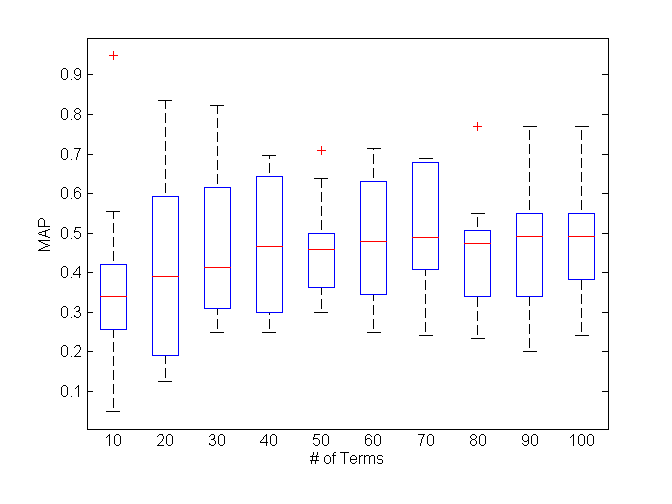
\includegraphics[trim=0cm 0cm 0cm 0cm, clip=false, totalheight=0.3\textheight, angle=0]{terms-map.png}%
\label{terms-map}} \hfil 
\subfigure[ P@5 Varying the Number of Terms ]{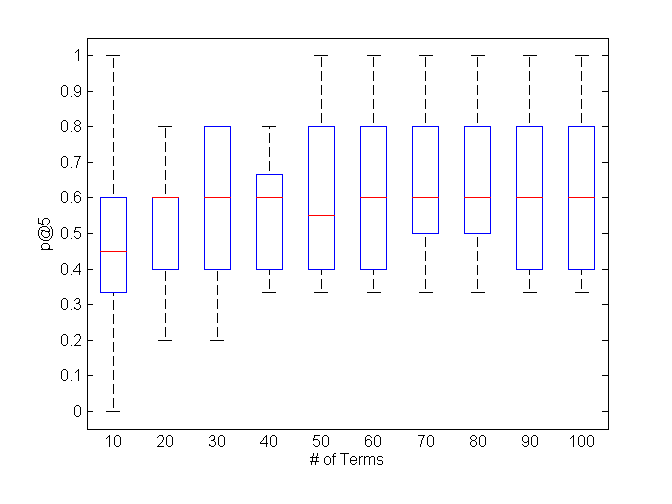
\includegraphics[trim=0cm 0cm 0cm 0cm, clip=false, totalheight=0.3\textheight, angle=0]{terms.png}%
\label{terms-p5}}} \caption{\textbf{Two different performance measure(MAP and P@5) were computed by varying the number of terms for our query generation. For these experiments the others parameters were as follows: $\alpha$ = 1.0, $\lambda$ = 0.9, $b$ = 0.1}} \label{terms}
\end{figure*}
\begin{figure*}[!ht]
\centering
\captionsetup{justification=centering}
{\subfigure[]{\includegraphics[trim=0cm 0cm 0cm 0cm, clip=false, totalheight=0.3\textheight, angle=0]{comparison-terms.png}%
\label{com-terms-map}} \hfil 
\subfigure[]{\includegraphics[trim=0cm 0cm 0cm 0cm, clip=false, totalheight=0.3\textheight, angle=0]{comparison-terms-p5.png}%
\label{com-terms-p5}}} \caption{\textbf{Performance Comparison of MAP and P@5 between the typical Okapi-BM25 algorithm and our modified Okapi-BM25 algorithm by varying the number of terms in a passage query}} \label{com-terms}
\end{figure*}
\begin{figure*}[!ht]
\centering
\captionsetup{justification=centering}
{\subfigure[]{\includegraphics[trim=0cm 0cm 0cm 0cm, clip=false, totalheight=0.3\textheight, angle=0]{comparison-terms-yahoo.png}%
\label{com-terms-map-yahoo}} \hfil 
\subfigure[]{\includegraphics[trim=0cm 0cm 0cm 0cm, clip=false, totalheight=0.3\textheight, angle=0]{comparison-terms-yahoo-p5.png}%
\label{com-terms-yahoo-p5}}} \caption{\textbf{Performance Comparison of MAP and P@5 between the typical Okapi-BM25 algorithm and our modified Okapi-BM25 algorithm by varying the number of terms in a passage query with Yahoo-news articles}} \label{com-terms}
\end{figure*}

In our System, from each passage of an article we generate a query representing the information need satisfied by the concerned passage of that article. If the number of terms in that query is too small, it may not cover all the concerned topics of an article. Also, if the numbers of terms are too many, it might become too generic. Figure \ref{terms-map} and Figure \ref{terms-p5} presents the impact of number of terms in the query on MAP and P@5 respectively.

Figure \ref{terms-map} shows that, the MAP generally increases with the increased number of terms in query. And we get the highest MAP for query with 70 terms. This is quite expected because with the increase in the number of terms generally more relevant comments are pulled out. However, for much higher number of terms the query becomes more general and hence more irrelevant documents are also pulled out so with more than 80 terms MAP suffers a little bit.
Figure \ref{terms-p5} shows that, the value of P@5 also generally increases with the increase in the number of terms in query. We get the highest value of P@5 when number of terms in query is 70 and 80. Also, the value of P@5 decreases for much higher number of terms in query for reasons mentioned above.  Hence, we chose the 70 terms for each query for the next set of experiments. 



\subsection{Modification on Okapi BM25}
One of the major drawback of using Okapi BM25 in our system, as described in the previous section, was that BM25 does not allow us to use the term probabilities of the query terms used for query generation. So, in this project along with normal BM25 algorithm we experimented with a little tweak on the Okapi BM25 equation. 

To incorporate the query term probabilities into the ranking function, we proposed a modification on the Okapi BM25 relevance equation. Here, the probability of a term's contributing to the query generated by the passage $P$ replaces the query term frequency component in the standard BM25 ranking formula given in Equation \ref{bm25} and gives us Equation \ref{modBM25}. 

\begin{widetext}
\begin{equation*}
\label{bm25}
rank(P,D) = \sum_{\substack{w \in P,D}}\log{\frac{N - df + 0.5}{df + 0.5}} \times 
{\frac{(k_1 + 1) \times c(w, D)}{k_1 \times (1 - b + b \frac{n}{n_{avg}}) + c(w,D)}} \times
\frac{(k_2 + 1) \times {c(w, P)}}{k_2 + c(w, P)}
\end{equation*}
\end{widetext}


\begin{widetext}
\begin{equation*}
\label{modBM25}
rank(P,D) = \sum_{\substack{w \in P,D}}\log{\frac{N - df + 0.5}{df + 0.5}} \times 
{\frac{(k_1 + 1) \times c(w, D)}{k_1 \times (1 - b + b \frac{n}{n_{avg}}) + c(w,D)}} \times p_p(w)
\end{equation*}
\end{widetext}


   

\subsection{Performance Measurement of the System}




\section{Limitation and Future Work}
\label{fw}
As we expressed before that our broad objective for the research was to develop a mechanism for classifying, filtering, and highlighting readers' comments; and we restrict it to only filtering relevant comments to fit our work within the time frame of the class project. Given that none of us works in Information Retrieval and has his personal research to do, it seems unlikely that our initial plan will come to fruition.

Nevertheless, we see several improvements possible in comments filtering alone that we could not address because of other engagements. We are interested to investigate these possibilities in the future if further work in this project seems worthwhile (depending on the feedback we may get). Below we discuss these potential improvements.       

\subsubsection{Changes in Comments Filtering Criteria}
Apart from doing a language based comments evaluation that we discussed before in Section \ref{si}, we can make two more changes that may change our solution's performance considerably. First, our observation suggests that comments filtering should be based on some minimum threshold of similarities instead of document ranking. This is because many news articles that we examined although having a lot of comments have only a few of them that are useful. The opposite is quite true also where there are few comments but all of make have meaningful contributions to the article. From the presentation perspective it might be better to remove incoherent comments altogether than doing just an ordering.

Second, we observed in articles with a huge number of comments (e.g., in the scale of hundreds), later comments tend to diverge greatly from the discussion of the article. It seems to be a common trend that after a few comments readers start commenting on one another's comments and embroil in personal arguments instead of addressing the content of the article. Therefore, it might worth a try to consider a comment's position and nesting level during ranking evaluation.            

\subsubsection{Get More Relevance Judgements}
We collected over 730 Yahoo-News articles from \cite{Das:2014:GBC:2556195.2556231} and crawled over 850 articles from Alzajeera News. These articles are comment rich and there are minimum 20 comments per article. Our evaluation is, however, done over a minute sample having less than 40 articles. This is a place where we definitely need to improve.  

We asked some friends and fellow researchers to read 5 to 10 random articles and provide relevance judgements for accompanying comments. Unfortunately, we got feedback for 1 or 2 articles per person -- sometimes we got none. We believe there was a lack of incentive in providing feedbacks as there was no accompanying reward. One good idea for collecting many relevance judgements can be to use something like Amazon Mechanical Turk with a reasonable remuneration per feedback. Further, we only asked for binary relevance judgements from our participants to make the task easy for them. In a formal feedback generation experiment, we can ask for graded relevance. We will then need some funding to undertake this experiment though.    

\subsubsection{Addressing Synonymy}
One obvious thing to do to improve performance further is to apply a synonym analyser based on some lexical dictionary tool such as WordNet \cite{Miller:1995:WLD:219717.219748} during both query language model construction and comments ranking. We observed several cases where a minor difference in the terminology used such as `Britain' as opposed `British' resulting in unwanted expansion of the query language model and loss of efficiency in comment filtering.    

\subsubsection{Further Experiment on Passage Determination} We could not do passage level comment filtering as our collection of articles seems to overwhelmingly lack any noticeable paragraph henceforth passage level decomposition. We suspect this is a characteristic of the two news sources we considered. Our experience of reading news from more renowned news sources such as New York Times and BBC News suggest that many interesting articles have good paragraph structures in them. 

We initially spent considerable time trying to crawl news from New York Times but could not determine how to crawl readers' comments from its articles. BBC News, we did not try at all. An interesting next step is to investigate how to crawl from these two and some other popular news sources where articles tend to be more structured and measure performance of passage level comments filtering. We believe using more popular news sources for analysis will boost up the significance of our work also.     
 
\section{Conclusion}
\label{con}
In this project, we developed, to the best of our knowledge, a novel technique for automatically filtering and classifying relevant readers' comments for newspaper articles. Such a solution should be greatly useful for newspaper readers and editors alike in an era where unrestricted commenting leads to a rapid increase of both useful and unwanted comments.

We treated an article title as a query and used that as a cue to develop structured query language models for the passages in that article where each term's probability of occurrence in a query generated from a model depends on values of several parameters such as its significance, number of co-occurrences with more important terms, and frequency. Then the task of selecting a relevant comment has been translated into a similarity matching problem between the comment's and article passage's language models. 

Due to time constraints, we had to settle for a prototype implementation of the solution that cut few corners here and there that we believe affected our solution's performance. Particularly, we could not manage enough time to learn and implement a model similarity based comments ranking function, and did ranking and filtering of comments using Okapi BM25. Without a synonymy checker and an ideal retrieval function the performance of our implementation is still very encouraging.

On a sample articles set annotated by human with binary relevance judgements, we achieved a MAP around 0.6 and P@5 over 0.5         even with all implementation shortcomings. This is a good enough result to be excited about and we are interested to take the project to the next step by enhancing our relevance judgements database, implementing a full fledged solution, and doing more evaluations. We just need some guidance and support along the way. 

\bibliographystyle{abbrv}
\bibliography{bibliography} 

\end{document}
